% !TeX encoding = UTF-8

\documentclass{protokol}

\usepackage{pdfpages}
\usepackage{tikz}
\usetikzlibrary{calc}
\usetikzlibrary{arrows}

%====== Units =====
\usepackage{siunitx}
\sisetup{inter-unit-product =\ensuremath{\cdot}}
\sisetup{group-digits = integer}
\sisetup{output-decimal-marker = {,}}
\sisetup{exponent-product = \ensuremath{\cdot}}
\sisetup{separate-uncertainty}
\sisetup{tight-spacing = false}
%\sisetup{scientific-notation = true}
%\sisetup{round-mode=places,round-precision=4}
%\sisetup{evaluate-expression}


%====== Grafy =====
\usepackage{pgfplots}
\pgfplotsset{width=0.8\linewidth, compat=1.17}
\def\plotcscale{0.8}
\usepackage{pgfplotstable}
\usepackage[figurename=Obr.]{caption} % figure caption rename

%====== Rovnice align block ======
\usepackage{amsmath}
\setlength{\jot}{10pt} % rozestup mezi řádky

\graphicspath{ {./img/} }

%====== Vyplňte údaje ======
\jmeno{Jakub Charvot}
\kod{240844}
\rocnik{3.}
\obor{MET}
\skupina{MET/2}
\spolupracoval{--}

\merenodne{19.02.\ 2024}
\odevzdanodne{25.02.\ 2024}
\nazev{Extrakce parametrů tranzistorů MOSFET ze SPICE modelu }
\cislo{1} %měřené úlohy

\predmet{Návrh analogových integrovaných obvodů}
\ustav{Ústav mikroelektroniky}
\skola{FEKT VUT v~Brně}

\def\para{x+0}
\def\parb{\para-80}


%citace 
\usepackage[backend=biber, style=iso-numeric, sortlocale=cs_CZ, autolang=other, language=czech]{biblatex}
\addbibresource{bibliography.bib}
\DeclareFieldFormat{labelnumberwidth}{\mkbibbrackets{#1}}
% hyperlinky
\usepackage[colorlinks]{hyperref}

% odstavce
\usepackage{parskip}

% Bloky kódu
\usepackage{xcolor}

%New colors defined below
\definecolor{codegreen}{rgb}{0,0.6,0}
\definecolor{codegray}{rgb}{0.5,0.5,0.5}
\definecolor{codepurple}{rgb}{0.58,0,0.82}
\definecolor{backcolour}{rgb}{0.95,0.95,0.92}

\usepackage{listings}
\lstdefinestyle{mystyle}{
  backgroundcolor=\color{backcolour}, commentstyle=\color{codegreen},
  keywordstyle=\color{magenta},
  numberstyle=\tiny\color{codegray},
  stringstyle=\color{codepurple},
  basicstyle=\ttfamily\footnotesize,
  breakatwhitespace=false,         
  breaklines=true,                 
  captionpos=b,                    
  keepspaces=true,                 
  numbers=left,                    
  numbersep=5pt,                  
  showspaces=false,                
  showstringspaces=false,
  showtabs=false,                  
  tabsize=2
}
\lstset{
	inputencoding=utf8,
	extendedchars=true,
	literate={á}{{\'a}}1 {č}{{\v{c}}}1 {ď}{{\v{d}}}1 {é}{{\'e}}1 {ě}{{\v{e}}}1 
           {í}{{\'i}}1 {ň}{{\v{n}}}1 {ó}{{\'o}}1 {ř}{{\v{r}}}1 {š}{{\v{s}}}1 
           {ť}{{\v{t}}}1 {ú}{{\'u}}1 {ů}{{\r{u}}}1 {ý}{{\'y}}1 {ž}{{\v{z}}}1 
           {Á}{{\'A}}1 {Č}{{\v{C}}}1 {Ď}{{\v{D}}}1 {É}{{\'E}}1 {Ě}{{\v{E}}}1 
           {Í}{{\'I}}1 {Ň}{{\v{N}}}1 {Ó}{{\'O}}1 {Ř}{{\v{R}}}1 {Š}{{\v{S}}}1 
           {Ť}{{\v{T}}}1 {Ú}{{\'U}}1 {Ů}{{\r{U}}}1 {Ý}{{\'Y}}1 {Ž}{{\v{Z}}}1,
	style=mystyle
	}

% Číslování
\pagenumbering{arabic}

% =========================================
% =============== DOKUMENT ================
% =========================================
\begin{document}
	%====== Vygenerování tabulky ======
	\maketitle

\section{Vypracování}
  Pro provedení všech simulací jsem použil dvě zapojení, jedno pro tranzistor typu NMOS (viz Obr.~\ref{fig:img-nmos-png}), druhé pak pro typ PMOS (Obr.~\ref{fig:img-pmos-png}). Napájecí uzly jsem definoval pro obě zapojení stejně, jako je vidět na třetím schématu na Obr.~\ref{fig:img-power-png}.

  SPICE kód potřebný pro simulace jsem rozdělil do několika bloků (viz Obr.~\ref{fig:img-spice-png}) a vždy přepínal mezi komentářem a spustitelným kódem. Díky tomu jsem omezil duplicitní kód a mohl využít obě schémata jednoduše pro všechny tři simulace, vždy s výběrem vhodné kombinace bloků. Bohužel s tímto konceptem možná drobně klesá přehlednost.

  \begin{figure}[h!]
    \centering
    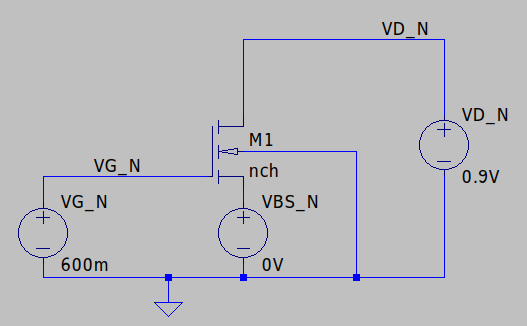
\includegraphics[scale=1]{img/nmos.png}
    \caption{Zapojení s tranzistorem NMOS.}
    \label{fig:img-nmos-png}
  \end{figure}

  \begin{figure}[h!]
    \centering
    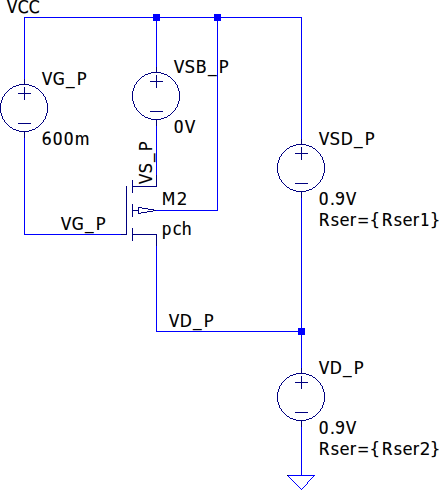
\includegraphics[scale=1]{img/pmos.png}
    \caption{Zapojení s tranzistorem PMOS.}
    \label{fig:img-pmos-png}
  \end{figure}

  \begin{figure}[h!]
    \centering
    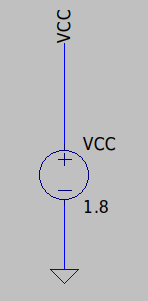
\includegraphics[scale=1]{img/power.png}
    \caption{Definice uzlů napájení pro zbylé obvody.}
    \label{fig:img-power-png}
  \end{figure}

  \begin{figure}[h!]
    \centering
    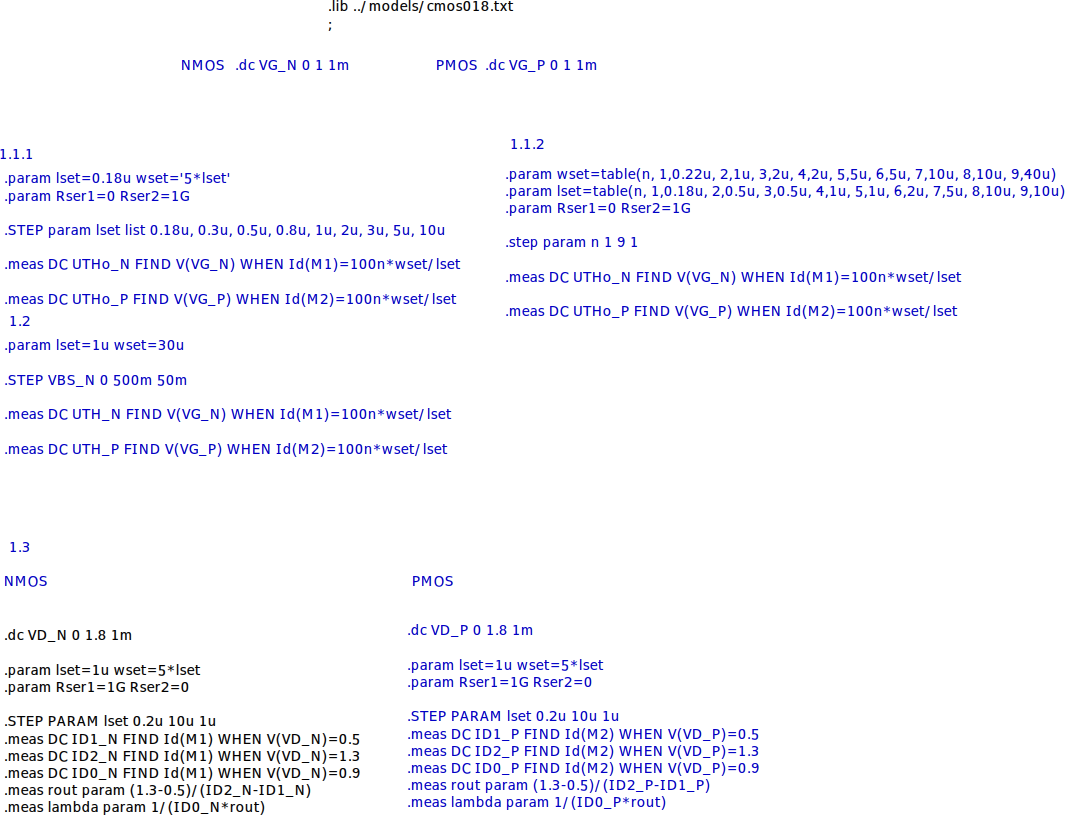
\includegraphics[width=\textwidth]{img/spice.png}
    \caption{Všechny použité bloky SPICE kódy.}
    \label{fig:img-spice-png}
  \end{figure}


  \clearpage
\subsection{Prahové napětí \(U_{TH0} \) }
\begin{table}[]
    \def\arraystretch{1.2}
    \centering
    \begin{tabular}{|l|l|l|l|}
    \hline
    L [\unit{\micro\meter}]    & W/L & \(U_{TH0 N}\) [mV] & \(U_{TH0 P}\) [mV] \\ \hline\hline
    0,18 & 5   & 417,456  & 470,74   \\ \hline
    0,3  & 5   & 434,41   & 465,15   \\ \hline
    0,5  & 5   & 418,739  & 458,1    \\ \hline
    0,8  & 5   & 396,187  & 448,17   \\ \hline
    1    & 5   & 386,941  & 443,4    \\ \hline
    2    & 5   & 368,024  & 432,03   \\ \hline
    3    & 5   & 362,038  & 428,07   \\ \hline
    5    & 5   & 357,358  & 425,05   \\ \hline
    10   & 5   & 353,717  & 423,13   \\ \hline
    \end{tabular}
    \caption{Prahové napětí podle 1.1.1.}
    \label{tab:1-1-1_hodnoty}
\end{table}

\begin{table}[]
    \def\arraystretch{1.2}
    \centering
    \begin{tabular}{|l|l|l|l|l|}
    \hline
    W [\unit{\micro\meter}]    & L [\unit{\micro\meter}]     & W/L  & \(U_{TH0 N}\) [mV] & \(U_{TH0 P}\) [mV] \\ \hline\hline
    0,22  & 0,18 & 1,22& 382,2  & 407,52   \\ \hline
    1    & 0,5  & 2    & 417,049   & 454,45   \\ \hline
    2    & 0,5  & 4    & 418,458  & 457,55    \\ \hline
    2    & 1    & 2    & 386,64  & 443,06   \\ \hline
    5    & 1    & 5    & 386,941  & 443,4    \\ \hline
    5    & 2    & 2,5  & 368,009  & 432,23   \\ \hline
    10   & 5    & 2    & 357,377  & 425,29   \\ \hline
    10   & 10   & 1    & 353,754  & 423,48   \\ \hline
    40   & 10   & 4    & 353,72  & 423,16   \\ \hline
    \end{tabular}
    \caption{Prahové napětí podle 1.1.2.}
    \label{tab:1-1-2_hodnoty}
\end{table}



\begin{figure}[h!]
    \centering
    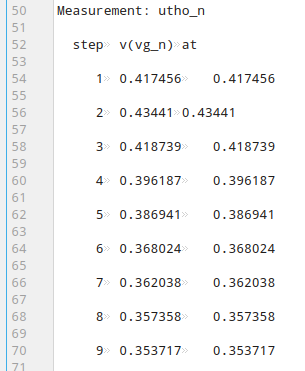
\includegraphics[]{img/log1.png}
    \caption{Ukázka SPICE output log.}
    \label{fig:img/log1.png}
\end{figure}


\begin{figure}[h!]
    \centering
    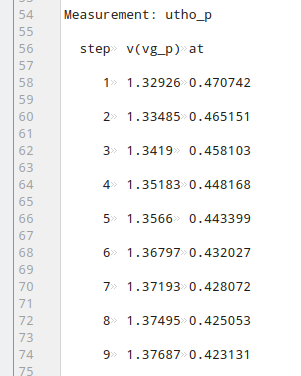
\includegraphics[]{img/log2.png}
    \caption{Ukázka SPICE output log.}
    \label{fig:img/log1.png}
\end{figure}

\begin{figure}[h!]
    \centering
    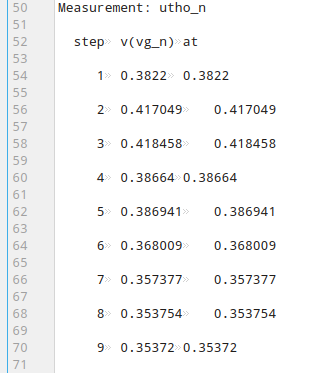
\includegraphics[]{img/log3.png}
    \caption{Ukázka SPICE output log.}
    \label{fig:img/log1.png}
\end{figure}

\begin{figure}[h!]
    \centering
    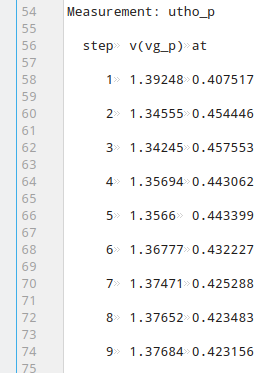
\includegraphics[]{img/log4.png}
    \caption{Ukázka SPICE output log.}
    \label{fig:img/log1.png}
\end{figure}



\clearpage
\subsection{Závislost prahového napětí \(U_{TH} \) na napětí bulku}
\begin{table}[]
    \def\arraystretch{1.2}
    \centering
    \begin{tabular}{|l|l|l|}
    \hline
    \(U_{SB} \) [V]  & \(U_{TH N}\) [mV] & \(U_{TH P}\) [mV] \\ \hline\hline
    0          & 387,106  & 443,3  \\ \hline
0,05           & 406,335  & 459,39  \\ \hline
    0,1        & 420,771  & 475,16  \\ \hline
0,15           & 434,894  & 490,64  \\ \hline
    0,2        & 448,718  & 505,85  \\ \hline
0,25           & 462,268  & 520,8  \\ \hline
    0,3        & 475,556  & 535,506  \\ \hline
0,35           & 488,6    & 549,989  \\ \hline
    0,4        & 501,413  & 564,254  \\ \hline
0,45           & 514,011  & 578,318  \\ \hline
    0,5        & 526,4    & 592,191  \\ \hline
    \end{tabular}
    \caption{Prahové napětí podle 1.2.}
    \label{tab:1-1-2_hodnoty}
\end{table}

\begin{figure*}[h!]
    \begin{tikzpicture}
        \centering
        \begin{axis}
            [
            xlabel={\( U_{SB/BS}\ [\unit{\volt}]\)},
            ylabel={\( U_{TH} \ [\unit{\milli\volt}]\)},
            width=1\textwidth,
            height = 0.5\textwidth,
            legend pos=north west,
%			xmin=0,
%			ymin=0,
%			xmax=100
%			ymax=100
            ]

            \addplot[mark=x, mark options={solid}, thick, red, mark size=3pt] table [x=USB, y=UTHN, col sep=comma] {data/1-2.csv};
            \addlegendentry{NMOS}
            
            \addplot[mark=x, mark options={solid}, thick, blue, mark size=3pt] table [x=USB, y=UTHP, col sep=comma] {data/1-2.csv};
            \addlegendentry{PMOS}
            
        \end{axis}       
    \end{tikzpicture}
    \caption{Závislost prahového napětí \(U_{TH N/P} \) na napětí na bulku. }
\end{figure*}


\clearpage
\subsection{Závislost modulace délky kanálu (\(\lambda\)) na délce kanálu \( L\) }
\begin{figure*}[h!]
    \begin{tikzpicture}
        \centering
        \begin{axis}
            [
            xlabel={\( L\ [\unit{\micro\meter}]\)},
            ylabel={\( \lambda\ [\unit{\per\volt}]\)},
            %axis y line*=left, % dve y osy
            width=1\textwidth,
            height = 0.5\textwidth,
            legend pos=north east,
%			xmin=0,
%			ymin=0,
%			xmax=100
%			ymax=100
            ]

            \addplot[mark=none, mark options={solid}, thick, red, solid, mark size=3pt] table [x=L, y=lambdan, col sep=comma] {data/1-3.csv};
            
            \addlegendentry{NMOS}

            \addplot[mark=none, mark options={solid}, thick, blue, solid, mark size=3pt] table [x=L, y=lambdap, col sep=comma] {data/1-3.csv};
            
            \addlegendentry{PMOS}
            
        \end{axis}   
     
    \end{tikzpicture}
    \caption{Závislost modulace délky kanálu na délce kanálu.}
\end{figure*}


\begin{table}[]
    \def\arraystretch{1.2}
    \centering
    \begin{tabular}{|l|l|l|}
    \hline
    \(L \) [\unit{\micro\meter}]  & \(\lambda_{NMOS} \) [\unit{\per\volt}] & \(\lambda_{PMOS} \) [\unit{\per\volt}] \\ \hline\hline
    0,50  & 0,118405  &  0,199965        \\ \hline
    0,80  & 0,0864604  &  0,144768       \\ \hline
    1,00  & 0,0744184  &  0,124192       \\ \hline
    1,20  & 0,0654639  &  0,109762       \\ \hline
    2,00  & 0,0437895  &  0,0787697      \\ \hline
    5,00  & 0,0186175  &  0,0459268      \\ \hline
\end{tabular}
\caption{Vypočítané hodnoty modulace délky kanálu dle 1.3.}
\label{tab:1-3_hodnoty}
\end{table}


\section{Závěr}
  V první části úlohy jsme stanovovali prahové napětí tranzistoru při zachování konstantníhi poměru délky a šířky kanálu. Z výsledků je vidět, že pro rostoucí délku kanálu prahové napětí klesá. V další podúloze jsme měnili poměr W/L, z čehož vyplynulo, že šířka kanálu W nemá na prahové napětí významný vliv, podstatnější je délka.

  Ve druhé části úlohy jsme neovlivňovali délku ani šířku kanálu, ale připojovali jsme napětí na bulk, tedy substrát tranzistoru, čímž jsme simulovali tzv. Body efekt. S nárustém napětí na bulku roste také prahové napětí tranzistoru. 

  V poslední části jsme počítali modulaci délky kanálu v závislosti na samotné délce kanálu. U obou typů tranzistorů s rostoucí délkou tranzistoru tento efekt klesá.

% \section*{Reference}
% \printbibliography[heading=none]


\end{document}